% !TEX root = Formulaire_fluides.tex

\appendix

\section{Propriétés physiques des fluides les plus courants}

(Valeurs de référence pour $T = 20^o C$ ; $P = 10^5 Pa = 1 atm$) 

\vspace{.5cm}

\begin{tabular}{|l|l|l|l|} 
\hline
					& Air 							& Eau pure 						& Eau de mer \\
\hline
Masse volumique & 		$\rho = 1.205 kg/m^3$				& $1000 kg/m^3$					&  $1027 kg/m^3$ \\
 Viscosité cin. & 		$\nu = 1.5e-6 m^2/s$ 				& $\nu = 1.188 \cdot 10^{-6} m /s^2$		&  $\nu = 1.139 10^{-6} m /s^2$ \\
 Viscosité dyn. & 		$\mu = 1.81 \cdot 10^{-5} Pa \cdot s$ 	& $\mu = 1.188\cdot  10^{-3} Pa \cdot s$ 	& \\
 compressibilité & 		$\chi_s = 1.4 atm^{-1}$ 				&$\chi_s =  4.9 \cdot 10^{-5} Atm^{-1}  	& \\
 dilatabilité & 			$ \alpha = 3.4 \cdot 10{-3} K^{-1}$  		& $ \alpha = 1.5 \cdot 10{-4} K^{-1}$  	& \\
 vitesse du son &		$ c = 334 m/s$ 						& $c = 1500 m/s$ 					& \\  
 \hline
\end{tabular}
%La masse volumique de l'eau vaut $\rho_M = 1000 kg/m^3$ pour le modèle
%et $\rho = 1026 kg/m^3$ pour le navire. La viscosité cinématique de l'eau est 
%$\nu_M = 1.139 10^{-6} m /s^2$ pour le modèle et $\nu = 1.188 10^{-6} m /s^2$
%pour le navire.



\subsubsection{ANNEXE : Equation d'état de l'eau de mer (IES80)}

La relation d'état IES80 permet  de calculer $\rho$ ($kg /m^3$) en fonction
de $T$ (température en  en $^o C$), $S$ (salinité en $g/kg$), et $P$ (pression en $Bars$). 

Elle est précise (en toute rigueur) pour $-2^oC<T < 40^o C$, $0<S<40g/kg$, 
$0<P<1500 Bars$.
{
\tiny

$$
\rho(T,S,P) = \rho_0(T,S) \left/ \left( 1 - \frac{P}{K(T,S,P)} \right) \right.,
$$

avec :

\begin{eqnarray*}
\rho_0(T,S) &=& 999.842594+6.793952\cdot 10^{-2} \times T-9.09529\cdot 10^{-3} \times T^2+1.001685\cdot 10^{-4} \times T^3 -1.120083\cdot 10^{-6} \times T^4 \\
            &+& 6.536332\cdot 10^{-9} \times T^5+8.24493\cdot 10^{-1} \times S-4.0899\cdot 10^{-3} \times T S+7.6438\cdot 10^{-5} \times T^2 S \\
	    &-&8.2467\cdot 10^{-7} \times T^3 S + 5.3875\cdot 10^{-9} \times T^4 S-5.72466\cdot 10^{-3} \times S^{1.5}+1.0227\cdot 10^{-4} \times T S^{1.5}\\
	    &-&1.6546\cdot 10^{-6} \times T^2 S^{1.5}+4.8314\cdot 10^{-4} \times S^2, 
\end{eqnarray*}

et 

\begin{eqnarray*}
K(T,S,P) &=& 19652.21+148.4206 \times T-2.327105 \times T^2+1.360447\cdot 10^{-2} \times T^3-5.155288\cdot 10^{-5} \times T^4 \\
         &+&3.239908 \times P+1.43713\cdot 10^{-3} \times T P+1.16092\cdot 10^{-4} \times T^2 P-5.77905\cdot 10^{-7} \times T^3 P \\
         &+&8.50935\cdot 10^{-5} \times P^2-6.12293\cdot 10^{-6} \times T P^2+5.2787\cdot 10^{-8} \times T^2 P^2 \\
         &+&54.6746 \times S-0.603459 \times T S+1.09987\cdot 10^{-2} \times T^2 S \\
         &-&6.1670\cdot 10^{-5} \times T^3 S+7.944\cdot 10^{-2} \times S^{1.5}+1.6483\cdot 10^{-2} \times T S^{1.5}-5.3009\cdot 10^{-4} \times T^2 S^{1.5} \\
         &+&2.2838\cdot 10^{-3} \times P S-1.0981\cdot 10^{-5} \times T P S-1.6078\cdot 10^{-6} \times T^2 P S \\
	 &+&1.91075\cdot 10^{-4} \times P  S^{1.5}-9.9348\cdot 10^{-7} \times P^2 S+2.0816\cdot 10^{-8} \times T P^2 S \\
	 &+&9.1697\cdot 10^{-10} \times T^2 P^2 S.
\end{eqnarray*}

}


\begin{landscape}

\section{Tableau des principaux nombres sans dimensions}

On note ici $U$, $L$ les échelles de vitesse et de longueur du problème, et (pour les problèmes instationnaires) $T$ l'échelle de temps imposée par les conditions limites.
% (par exemple l'inverse de la fréquence d'oscillation).

\vspace{.5cm}

\begin{tabular}{|l   |l    |c    |l   |}
\hline
Nom & Définition & Signification & Utilité \\
\hline 
\hline
&&&\\
\color{red}{Knudsen} & 
$Kn = \frac{\ell}{L}$ & 
$\displaystyle\frac{ \mbox{échelle microscopique}}{ \mbox{échelle macroscopique}}$ &
Validité de la MMC
\\
&&&\\
\hline
&&&\\
Reynolds & $Re = \frac{U L}{\nu} $& 
$\displaystyle\frac{ \mbox{effets d'inertie}}{ \mbox{effets visqueux}}$ &
Général
\\
&&&\\
\hline
&&&\\
Mach & $Ma = \frac{U }{c}$ & 
$\displaystyle\frac{ \mbox{Vitesse de l'écoulement}}{ \mbox{vitesse du son}}$ &
Aérodynamique
\\
&&&\\
\hline
&&&\\
Froude & $Re = \frac{U }{\sqrt{gL}}$ & 
 $\displaystyle \frac{ \mbox{accélération dans l'écoulement}}{ \mbox{accélération de pesanteur}}$ &
Hydrodynamique, écoulements à surface libre
\\
&&&\\
\hline
&&&\\
Bond
  & $Bo = \frac{L}{\sqrt{\gamma/\rho g}}$  & 
$\color{red}{\frac{ \mbox{Effets de pesanteur}}{ \mbox{Effets capillaires}}}$ &
Phénomènes capillaires
\\
\color{red}{(ou E\"otv\"os)} &&&\\
%\hline
%&&&\\
%Gallilée & $Ga = \frac{\sqrt{g L^3}}{\nu}$ & 
%$\displaystyle\frac{ \mbox{Effets de gravité}}{ \mbox{Effets visqueux}}$ &
%Objets en mouvement libre dans un fluide
%\\
%&&&\\
\hline
&&&\\
Stokes
 & $St =  \frac{L^2}{\nu T }$ & 
$\displaystyle\frac{ \mbox{Effets instationnaires}}{ \mbox{Effets visqueux}}$ &
Ecoulements visqueux instationnaires
\\
(ou Womerseley)  &&&\\
\hline
&&&\\
Strouhal
 & $Sr =  \frac{L}{U T} $ & 
$\displaystyle\frac{ \mbox{Effets instationnaires}}{ \mbox{\color{red}{Effets inertiels}}}$ &
Ecoulements inertiels instationnaires
\\
&&&\\
\hline
&&&\\
Helmholtz
 & $H =  \frac{L}{c T} $ & 
$\displaystyle\frac{ \mbox{Longueur caractéristique}}{ \mbox{longueur d'onde acoustique}}$ &
Acoustique
\\
&&&\\
\hline
\end{tabular}

\end{landscape}



\section{Equations-bilan sous forme locale et intégrale}

Dans cette annexe on résume les équations-bilan de la mécanique des fluides sous forme {\em locale } (equations différentielles gouvernant l'évolution temporelle des quantités locales) puis sous forme {\em intégrale } en considérant un volume de contrôle {\em Fixe} noté $\Omega$ de frontière 
$\partial \Omega$.
 

%\subsection{ Equations générales} 
%(...)

On considère ici le cas général d'un fluide Newtonien soumis à une force {\em massique} $\vec f$ (en général la pesanteur). On ne fait pas d'hypothèse sur le caractère compressible ou incompressible. En revanche on suppose la viscosité $\mu$ constante (ainsi que la conductivité thermique $k$), et on néglige la viscosité en volume $\mu''$.

Il existe de nombreuses variantes de ces équations-bilan, on liste ici les plus utiles. Un grand nombre d'autres formes sont données dans le livre {\em Mécanique des Fluides, Candel (Dunod)}.

%%%%%%%%%%%%%%%%%%%%%%%%%%%%%%
\subsection{Bilan de masse}

\begin{equation}
\mbox{\bf Forme locale 1 (non conservative)  :} 
\qquad  
\ddt{\rho} + \rho \divergence \vec{u} = 0
\end{equation}

\begin{equation}
\mbox{\bf Forme locale 2 (conservative) :}
\qquad  
\dpa{\rho}{t} + \divergence ( \rho \vec{u})  = 0
\end{equation}

\begin{equation}
\mbox{\bf Forme intégrale : } 
\qquad  
\ddt{} \int_{\Omega}  \rho dV = - \oint_{\partial \Omega} \rho \vec{u} \cdot \vec{n} dS
\end{equation}

% % bilan integral, volume matériel
% $$
%\dpdt{} \int_{\Omega} \rho \; dV 
%		=
%		- \oint_{\partial \Omega} \rho \,  \vec{u}\cdot \vec{n} \, dS
%$$

%%%%%%%%%%%%%%%%%%%%%%%%%%%%%%%%%%%%%
\subsection{Bilan de quantité de mouvement}

%\paragraph{Forme locale 1}
\begin{equation}
\mbox{\bf Forme locale 1 (non conservative)  :} 
\qquad  
		\rho \ddt{\vec{u}} 
		= 
		\rho \vec{f}  - \gradient p + \mu \Delta \vec{u} + \frac{\mu}{3} \gradient \divergence \vec{u} 
		%\label{eq:bilan_local_lagrangien_qdm}
\end{equation}
	
	
%\paragraph{Forme locale 2 (conservative)}
%\mbox{\bf Forme locale 2 (conservative) :}
%\qquad  

\begin{equation}
\mbox{\bf Forme locale 2 (conservative) :}
\qquad  
	 \dpa{(\rho \vec{u})}{t} + \divergence (\rho \vec{u} \otimes \vec{u})
		= \rho \vec{f}  - \gradient p + \divergence \mytensor{\tau}
		%\label{eq:bilan_local_lagrangien_qdm}
\end{equation}

\paragraph{Forme intégrale}
	\begin{equation}
		\ddt{} \int_{\Omega} \rho \, \vec{u} \; dV 
		=
		- \oint_{\partial \Omega} \rho \, \vec{u}\; (\vec{u}\cdot \vec{n}) \, dS
		+ \oint_{\partial \Omega} \left( -p \vec{n} + \mytensor{\tau} \cdot \vec{n}\right) \; dS
		+ \int_{\Omega} \rho \vec{f} \, dV 
		\left[ + \oint_{\cal L} \gamma \vec{t}  \, d\ell \right]
		\label{eq:bilan_global_eulerien_qdm}
	\end{equation}
	
{\small (Le dernier terme entre crochets est à prendre en compte si le volume de contrôle $\Omega$ est traversé par une {\em surface libre} ${\cal S}$ ; dans ce cas  $ {\cal L} = {\partial \Omega} \cap \cal S$ et $\vec t$ est le vecteur unitaire contenu dans le plan ${\cal S}$ et perpendiculaire à ${\cal L}$)}

%%%%%%%%%%%%%%%%%%%%%%%%%%%%%
\subsection{Bilan d'énergie cinétique}


\paragraph{Forme locale 1}
\begin{equation}
		\rho \ddt{} \frac{ |\vec{u}|^2}{2} 
		= 
		- \rho \vec{f} \cdot \vec{u}  - \gradient p \cdot {\vec u} + \vec{u} \cdot \divergence ( \mytensor{\tau} )
		%\label{eq:bilan_local_lagrangien_qdm}
\end{equation}

\paragraph{Forme locale 2}

$\,$
Sous les hypothèses suivantes :
\begin{itemize}
\item 
Le champ de force massique $\vec f$ est conservatif, c.a.d. 
$\vec f = -\gradient {\cal U}$ (en général ${\cal U}= g z$),
\item  Le fluide est barotrope (c.a.d. $p=p(\rho)$)\footnote{Cette notion englobe fluide incompressible pour lequel ${\cal P} = p/ \rho$  ainsi que le gaz parfait en évolution isotherme ou isentropique};

Dans ce cas on peut définir la  fonction 
%$\cal P$ telle que %$\rho^{-1} \gradient p=  \gradient {\cal P}$
${\cal P} = \int \frac{d p}{\rho}$, ce qui conduit à la formule suivante :
\end{itemize}

\begin{equation}
		\rho \dpdt{} \frac{ |\vec{u}|^2}{2} 
		+ \rho \vec{u} \cdot \gradient \left( \frac{ |\vec{u}|^2}{2} + {\cal U} +  {\cal P} \right) 
		= 
		 \vec{u} \cdot \divergence ( \mytensor{\tau} ) \textcolor{red}{= \divergence ( \vec{u} \cdot \mytensor{\tau} ) - \mytensor{D} :\mytensor{\tau}}
		%\label{eq:bilan_local_lagrangien_qdm}
\end{equation}

(on reconnait comme cas particulier le premier théorème de Bernoulli).



\paragraph{Forme intégrale}
	\begin{equation}
		\ddt{} \int_{\Omega} \frac{\rho |\vec{u}|^2}{2} \, dV 
		= -  \oint_{\partial \Omega} \left( \frac{\rho |\vec{u}|^2}{2} + p + \rho {\cal U} \right)  \cdot \vec u \, dS
		+ \int_{\Omega} p \, \divergence (\vec{u}) \, dV 
%		+ \int_{\Omega} \vec{u} \cdot \divergence ( \mytensor{\tau} ) \; dV
+ \textcolor{red}{ \oint_{\partial \Omega}  \vec{u} \cdot \mytensor{\tau} \cdot \vec{n} \, dS
 -  \int_{\Omega} \tensor{D} : \mytensor{\tau}  \, dV}	
		\label{eq:bilan_global_eulerien_ec}
	\end{equation}


\subsection{Bilan d'énergie (1er principe)}

Dans ce paragraphe $e$ est l'énergie interne {\em massique}\footnote{ $e = c_v T$ pour un gaz parfait}, $h = e+p/\rho$ est l'enthalpie massique\footnote{ $h = c_p T$ pour un gaz parfait}, $H$ est l'enthalpie totale, et $\vec q$ est le flux de chaleur conductif\footnote{ Donné en général par la loi de Fourier $\vec{q}=-k \gradient T$ }  

\paragraph{Forme intégrale 1}
\begin{equation}
		\underbrace{\ddt{} \int_{\Omega} \rho \left( e + \frac{ |\vec{u}|^2}{2} \right) \; dV
		}_{\ddt{E} }		 
		= \underbrace{  - \oint_{\partial \Omega}  \rho \left( e + \frac{ |\vec{u}|^2}{2} \right) \vec{u} \cdot \vec{n} \; dS
		}_{\dot{E}^{(ech)}}
		+ \underbrace{\int_{\Omega} \rho \vec{f} \cdot \vec{u} \; dV
		}_{\dot{W}^{(f)}} 
		+ \underbrace{ \oint_{\partial \Omega} -p \vec{u} \cdot  \vec{n}   \; dS 
		}_{\dot{W}^{(p)}} 
		+ \underbrace{ \oint_{\partial \Omega} \vec{u} \cdot  \mytensor{\tau} \cdot \vec{n}  \; dS 
		}_{\dot{W}^{(v)}} 
		 \underbrace{ - \oint_{\partial \Omega} \vec{q} \cdot \vec{n} \; dS
		}_{\dot{Q}} 
		\label{eq:bilan_global_eulerien_e1}
\end{equation}

\paragraph{Forme intégrale 2 (1er principe en système ouvert)}
\begin{equation}
		\underbrace{
		\ddt{} \int_{\Omega} \rho \left( h + \frac{ |\vec{u}|^2}{2} + {\cal U} \right) \; dV
		 }_{\ddt{H} }	
		= \underbrace{-  \oint_{\partial \Omega}  \rho \left( h + \frac{ |\vec{u}|^2}{2} + {\cal U} \right) \vec{u} \cdot \vec{n} \; dS
		}_{\dot{H}^{(ech)}} 
		+ \underbrace{ \int _{\Omega} \dpdt{p}\; dS
		}_{ V \ddt{P}  } 
		+ \underbrace{ \oint_{\partial \Omega} \vec{u} \cdot \mytensor{\tau} \cdot \vec{n}   \; dS 
		}_{\dot{W}^{(v)}} 
		 \underbrace{ - \oint_{\partial \Omega} \vec{q} \cdot \vec{n} \; dS
		}_{\dot{Q}} 
		\label{eq:bilan_global_eulerien_e2}
\end{equation}

Remarque : si le volume de contrôle ${\Omega}$ contient une surface intérieure ${\partial \Omega}_i$ mobile,
il convient d'ajouter
$$
W^{(utile)} = \int_{{\partial \Omega}_i}  \vec{u} \cdot \left( -p \vec{n}  \cdot  \mytensor{\tau} \cdot \vec{n} \right)  \; dS
$$ 



%\paragraph{Forme locale}
%\begin{equation}
%		\rho \ddt{} \left( \frac{ |\vec{u}|^2}{2} 
%		= 
%		- \rho \vec{f} \cdot \vec{u}  - \gradient p \cdot {\vec u} + \vec{u} \cdot \divergence ( \mytensor{\tau} )
		%\label{eq:bilan_local_lagrangien_qdm}
%\end{equation}


%\paragraph{Forme locale 1 }
\begin{equation}
\mbox{\bf Forme locale 1 :} \qquad 
		\rho \ddt{} \left( e+ \frac{|\vec{u}|^2}{2} \right) 
		= -\rho \vec{f} \cdot \vec{u} 
		- \gradient ( p) \cdot  \vec{u}  
		+ \divergence ( \mytensor{\tau}) \cdot \vec{u}  
		 - \divergence(\vec{q})
		%\label{eq:bilan_local_lagrangien_qdm}
\end{equation}



%\paragraph{Forme locale 2 }
\begin{equation}
\mbox{\bf Forme locale 2 :} \qquad 
		\rho \ddt{} \left( h + \frac{|\vec{u}|^2}{2} + {\cal U} \right) 
		=
		 \dpdt{p}
		+ \divergence ( \mytensor{\tau}) \cdot \vec{u}  
		 - \divergence(\vec{q})
		%\label{eq:bilan_local_lagrangien_qdm}
\end{equation}


\subsection{Bilan d'énergie interne}
Celui-ci s'obtient en combinant les deux précédents, et en écrivant la puissance des forces 
visqueuses comme la somme d'une puissance externe et d'une puissance interne :
$ \vec{u} \cdot \divergence ( \mytensor{\tau} ) =  \divergence ( \mytensor{\tau} \cdot \vec{u} ) -  \mytensor{\tau} : \mytensor{grad}(\vec{u})$. 


\paragraph{Forme locale}

\begin{equation}
		\rho \ddt{e} 
		= \mytensor{\tau} : \mytensor{grad}(\vec{u}) + 
		p \divergence( \vec{u})
		 - \divergence(\vec{q})
		%\label{eq:bilan_local_lagrangien_qdm}
\end{equation}


\paragraph{Forme intégrale}
	\begin{equation}
		\ddt{} \int_{\Omega} \rho e \; dV 
		= 
		- \int_{\Omega} p \, \divergence (\vec{u}) \; dV 
		+ \int_{\Omega} \mytensor{\tau} : \mytensor{grad}(\vec{u})  \; dV
		- \oint_{\partial \Omega} \vec{q} \cdot \vec{n} \; dS
		\label{eq:bilan_global_eulerien_e}
	\end{equation}


\subsection{Bilan d'entropie}

S'obtient a partir du bilan d'energie interne en posant $de = Tds - p d (1/\rho)$ :

%\paragraph{Forme locale}


\begin{equation}
\mbox{\bf Forme locale :} \qquad
		\rho \ddt{s} 
		=
		\frac{\mytensor{\tau} : \mytensor{grad}(\vec{u})}{T}
		 - \frac{\divergence(\vec{q})}{T}
		%\label{eq:bilan_local_lagrangien_qdm}
\end{equation}

\paragraph{Forme intégrale (second principe en système ouvert)}
\begin{equation}
		\underbrace{\ddt{} \int_{\Omega} \rho s \; dV
		}_{\ddt{S} }		 
		= \underbrace{  - \oint_{\partial \Omega}  \rho s \vec{u} \cdot \vec{n} \; dS
		}_{\dot{S}^{(ech)}}
		+ 
		\underbrace{ \int_{\Omega} \left( \frac{\mytensor{\tau} : \mytensor{grad}(\vec{u})}{T} + \vec{q} 		\cdot \frac{\gradient(T)}{T^2} 
		\right)   \; dS 
		}_{\dot{S}^{(cree)}} 
		 \underbrace{ - \oint_{\partial \Omega} \frac{\vec{q}}{T} \cdot \vec{n} \; dS
		}_{\dot{S}^{(recu)}} 
		\label{eq:bilan_global_eulerien_s}
\end{equation}








%--------------------------------------------------------------------------------------------------
\section{Opérateurs différentiels et équations de Navier-Stokes incompressibles dans les principaux systèmes de coordonnée}
%--------------------------------------------------------------------------------------------------




%On consid\`ere ici l'\'ecoulement incompressible d'un fluide newtonien,
%de viscosit\'e cin\'ematique $\nu = \mu / \rho$, soumis \`a la force volumique $\vec{f}$.

%\paragraph{Equations de Navier-Stokes}

%$$
%\dpa{\vec{u}}{t} + \left(\vec{u} \cdot \vec{grad} \right) \vec{u}
%=
%\frac{1}{\rho} \vec{f} - \frac{1}{\rho} \vec{grad} \, p + \nu \Delta \vec{u}
%$$

%\paragraph{Ecoulement incompressible}

%$$
%\mbox{div} \, \vec{u} = 0
%$$

%\paragraph{Tenseur des contraintes}

%$$
%\tensor{\sigma} = -p \tensor{1} + \tensor{\tau}
%\quad \mbox{avec} \quad
%\tensor{\tau} = 2 \mu \! \tensor{D} \, =
%\mu \left( \tensor{grad} \, \vec{u} +\, ^t\!\! \tensor{grad} \, \vec{u} \right )
%$$

%-------------------------------------------------------------------------------
\subsection{Coordonn\'ees cart\'esiennes $(x,y,z)$}


\paragraph{Divergence}
$$
\divergence (\vec{u}) = \dpa{u_x}{x} + \dpa{u_y}{y} + \dpa{u_z}{z}
$$


\paragraph{Vorticité}

\begin{eqnarray*}
\rot \vec{u} &=&  \left\{ 
\begin{array}{c} 
\displaystyle \omega_x = \dpa{u_z}{y}- \dpa{u_y}{z}\\
\displaystyle \omega_y = \dpa{u_x}{z}- \dpa{u_z}{x}\\
\displaystyle \omega_z = \dpa{u_y}{z}- \dpa{u_z}{y}\\
\end{array}
\right.
\end{eqnarray*}


\paragraph{Tenseur des contraintes}

\begin{eqnarray*}
\sigma_{xx} & = & -p + 2\mu \dpa{u_x}{x} \qquad \qquad 
\sigma_{xy} = \mu \left ( \dpa{u_x}{y} + \dpa{u_y}{x} \right ) \\
\sigma_{yy} & = & -p + 2\mu \dpa{u_y}{y} \qquad \qquad 
\sigma_{yz} = \mu \left ( \dpa{u_y}{z} + \dpa{u_z}{y} \right ) \\
\sigma_{zz} & = & -p + 2\mu \dpa{u_z}{z} \qquad \qquad 
\sigma_{xz} = \mu \left ( \dpa{u_z}{x} + \dpa{u_x}{z} \right ) 
\end{eqnarray*}



\paragraph{Equations de Navier-Stokes (écoulement incompressible)}

\begin{eqnarray*}
\dpa{u_x}{t} + u_x \dpa{u_x}{x} + u_y \dpa{u_x}{y} + u_z \dpa{u_x}{z} & = &
\frac{1}{\rho} f_x - \frac{1}{\rho} \dpa{p}{x}
+ \nu \left ( \ddpa{u_x}{x} + \ddpa{u_x}{y} + \ddpa{u_x}{z} \right )
\\ & & \\
\dpa{u_y}{t} + u_x \dpa{u_y}{x} + u_y \dpa{u_y}{y} + u_z \dpa{u_y}{z} & = &
\frac{1}{\rho} f_y - \frac{1}{\rho} \dpa{p}{y}
+ \nu \left ( \ddpa{u_y}{x} + \ddpa{u_y}{y} + \ddpa{u_y}{z} \right )
\\ & & \\
\dpa{u_z}{t} + u_x \dpa{u_z}{x} + u_y \dpa{u_z}{y} + u_z \dpa{u_z}{z} & = &
\frac{1}{\rho} f_z - \frac{1}{\rho} \dpa{p}{z}
+ \nu \left ( \ddpa{u_z}{x} + \ddpa{u_z}{y} + \ddpa{u_z}{z} \right )
\end{eqnarray*}


\paragraph{Fonction de courant $\psi$ } pour un écoulement incompressible plan 
($\vec{u} = u_x(x,y) \vec{e_x} + u_y(x,y) \vec{e_y}$)


\begin{equation}
 \vec{u} = \rot (\psi(x,y) \vec{e_z}), 
\quad \mbox{ c.a.d :} \quad \quad 
\left\{
\begin{array}{ccc}
 u_x &=& \displaystyle \dpa{\psi}{y}, \\
 u_y &=& \displaystyle -\dpa{\psi}{x}.
\end{array}
\right.
\end{equation}







\clearpage


%==================================================================================================
\subsection{Coordonn\'ees cylindriques ($r,\theta,z$)}
%==================================================================================================

\vspace{5mm}

\paragraph{Opérateurs différentiels}

%\paragraph{Divergence}

$$
\divergence (\vec{u}) = \frac{1}{r} \dpa{(r u_r)}{r} + \frac{1}{r} \dpa{u_{\theta}}{\theta} + \dpa{u_z}{z}\qquad 
%$$
%\paragraph{Vorticité}
%\begin{eqnarray*}
%\begin{array}{rcl}
\rot \vec{u} =  \left\{ 
\begin{array}{l} 
\displaystyle \omega_r = \left(\frac{1}{r}\frac{\partial \mathrm{u}_z}{\partial \theta} - \frac{\partial \mathrm{u}_\theta}{\partial z}\right) \\ \\
\color{red}{
\displaystyle \omega_\theta = \left(\frac{\partial \mathrm{u}_r}{\partial z} - \frac{\partial \mathrm{u}_z}{\partial r}\right) }
\\ \\
\displaystyle \omega_z = \frac{1}{r}\left(\frac{\partial}{\partial r}(r \mathrm{u}_\theta) - \frac{\partial \mathrm{u}_r}{\partial \theta}\right)\\
\end{array}
\right.
%\end{array}
$$

$$
\vec{grad} f = 
 \left\{ 
\begin{array}{l} 
\displaystyle \frac{\partial f}{\partial r} \\ \\
\displaystyle \frac{1}{r} \frac{\partial f}{\partial \theta} \\ \\
\displaystyle \frac{\partial f}{\partial z} \\
\end{array}
\right.
\qquad 
\Delta f = \frac{1}{r} \dpa{}{r} \left( r \dpa{f}{r} \right) + \frac{1}{r^2}\dpa{^2 f}{\theta^2} + \dpa{^2 f}{z^2}
$$

%\paragraph{Tenseur gradient des vitesses}

$$
\displaystyle
\tensor{grad} \left( \vec{u} \right) = \vec{\nabla} \otimes \vec{u}  =\overline{\overline{\nabla u}}=
\begin{bmatrix}
\displaystyle \frac{\partial u_r}{\partial r} & \displaystyle \frac{1}{r} \left( \frac{\partial u_r}{\partial \theta} - u_\theta \right) & \displaystyle \frac{\partial u_r}{\partial z} \\
\frac{\partial u_\theta}{\partial r} & \displaystyle \frac{1}{r} \left( \frac{\partial u_\theta}{\partial \theta} + u_r \right) & \displaystyle \frac{\partial u_\theta}{\partial z} \\
\displaystyle \frac{\partial u_z}{\partial r} & \displaystyle \frac{1}{r} \frac{\partial u_z}{\partial \theta} & \displaystyle \frac{\partial u_z}{\partial z}
\end{bmatrix}
$$

%
%\paragraph{Tenseur des contraintes}
%
%
%
%
%\begin{eqnarray*}
%\sigma_{rr} & = & -p + 2\mu \dpa{u_r}{r} \qquad \qquad \qquad \qquad %\qquad
%\sigma_{r\theta} = \mu \left( \frac{1}{r} \dpa{u_r}{\theta} + \dpa{u_{\theta}}{r} - \frac{u_{\theta}}{r} \right) \\
%\sigma_{\theta \theta} & = & -p + 2\mu \left( \frac{1}{r}\dpa{u_\theta}{\theta} + \frac{u_r}{r} \right) \qquad \quad
%\sigma_{\theta z} = \mu \left( \dpa{u_\theta}{z} + \frac{1}{r} \dpa{u_z}{\theta}\right) \\
%\sigma_{zz} & = & -p + 2\mu \dpa{u_z}{z} \qquad \qquad \qquad \qquad %\qquad
%\sigma_{rz} = \mu \left ( \dpa{u_z}{r} + \dpa{u_r}{z} \right ) 
%\end{eqnarray*}





\paragraph{Equations de Navier-Stokes (écoulement incompressible)}

\begin{eqnarray*}
\dpa{u_r}{t} + u_r \dpa{u_r}{r} + \frac{u_{\theta}}{r} \dpa{u_r}{\theta} + u_z \dpa{u_r}{z} - \frac{u_{\theta}^2}{r} & = &
\frac{1}{\rho} f_r - \frac{1}{\rho} \dpa{p}{r} \\
& + & \nu \left[ \frac{1}{r} \dpa{}{r} \left( r \dpa{u_r}{r} \right) + 
             \frac{1}{r^2} \ddpa{u_r}{\theta} + \ddpa{u_r}{z} -
             \frac{u_r}{r^2} - \frac{2}{r^2} \dpa{u_{\theta}}{\theta} \right] \\
\\
\dpa{u_{\theta}}{t} + u_r \dpa{u_{\theta}}{r} + \frac{u_{\theta}}{r} \dpa{u_{\theta}}{\theta} + u_z \dpa{u_{\theta}}{z} + \frac{u_r u_{\theta}}{r} & = &
\frac{1}{\rho} f_{\theta} - \frac{1}{\rho r} \dpa{p}{\theta} \\
& + & \nu \left[ \frac{1}{r} \dpa{}{r} \left( r \dpa{u_{\theta}}{r} \right) + 
             \frac{1}{r^2} \ddpa{u_{\theta}}{\theta} + \ddpa{u_{\theta}}{z} -
             \frac{u_{\theta}}{r^2} + \frac{2}{r^2} \dpa{u_r}{\theta} \right] \\
\\
\dpa{u_z}{t} + u_r \dpa{u_z}{r} + \frac{u_{\theta}}{r} \dpa{u_z}{\theta} + u_z \dpa{u_z}{z} & = &
\frac{1}{\rho} f_z - \frac{1}{\rho} \dpa{p}{z} \\
& + & \nu \left[ \frac{1}{r} \dpa{}{r} \left( r \dpa{u_z}{r} \right) + 
             \frac{1}{r^2} \ddpa{u_z}{\theta} + \ddpa{u_z}{z} \right]
\end{eqnarray*}


\paragraph{Fonction de courant $\psi$}  pour un écoulement incompressible plan exprimé en coordonnées polaires :

($\vec{u} = u_r(r,\theta) \vec{e_r} + u_\theta(r,\theta) \vec{e_\theta}$)


\begin{equation}
 \vec{u} = \rot (\psi(r,\theta) \vec{e_z}), 
\quad \mbox{ c.a.d :} \quad \quad 
\left\{
\begin{array}{ccc}
\displaystyle u_r &=& \displaystyle \frac{1}{r}\dpa{\psi}{\theta}, \\ \\
\displaystyle u_\theta &=&  \displaystyle -\dpa{\psi}{r}.
\end{array}
\right.
\end{equation}


\paragraph{Fonction de Stokes $\Psi$}  pour un écoulement à symétrie de révolution

($\vec{u} = u_r(r,z) \vec{e_r} + u_z(r,z) \vec{e_z}$)


\begin{equation}
% \vec{u} = \rot ( \Psi(x,y)/r  \vec{e_z}), 
%\quad \mbox{ c.a.d :} \quad \quad 
\left\{
\begin{array}{ccc}
\displaystyle u_r &=& \displaystyle - \frac{1}{r}\dpa{\Psi}{z}, \\ \\
\displaystyle u_z &=& \displaystyle  \frac{1}{r}\dpa{\Psi}{r}.
\end{array}
\right.
\end{equation}

% attention :  dans Guyon-Hulin-Petit : u_r = + ; u_z = -;
% dans Darrozes & Francois c'est l'opposé !



\clearpage

\subsection{Coordonnées sphériques $(R,\Theta,\phi)$}

\paragraph{Ecoulement incompressible}

$$\divergence(\vec{u})=\frac{\partial u_r}{\partial r} + 2 \frac{u_r}{r} + \frac{1}{r} \frac{\partial u_\theta}{\partial \theta} + \frac{1}{r \sin \theta} \frac{\partial u_\varphi}{\partial \varphi} + \frac{1}{\tan \theta} \frac{u_\theta}{r} 
$$

\paragraph{Equation de Navier-Stokes :}




\begin{eqnarray*}
\dpa{u_r}{t} + u_r \dpa{u_r}{r} 
+\frac{1}{r} \left[ 
 	\frac{u_{\theta}}{r} \dpa{u_r}{\theta} 
	+ \frac{u_{\varphi}}{sin \theta} \dpa{u_r}{\varphi} 
	- u_{\theta}^2 - u_{\varphi}^2
	\right] 
& = &
\frac{1}{\rho} f_r - \frac{1}{\rho} \dpa{p}{r} +  \nu \Delta_r \vec{u};
\\
\dpa{u_{\theta}}{t} 
+ u_r \dpa{u_{\theta}}{r} 
+ \frac{1}{r} \left[ 
		\frac{u_{\theta}}{r} \dpa{u_{\theta}}{\theta} 
		+ \frac{u_{\varphi}}{sin \theta} \dpa{u_r}{\varphi} 
		+ u_\theta u_\varphi - \frac{u_\varphi^2}{tan \theta} 
		+ u_\varphi \dpa{u_{\theta}}{\varphi} + \frac{u_r u_{\theta}}{r}
		\right] 
& = &
\frac{1}{\rho} f_{\theta} - \frac{1}{\rho r} \dpa{p}{\theta} 
 +  \nu \Delta_\theta \vec{u}; 
 \\
\dpa{u_\varphi}{t} + u_r \dpa{u_\varphi\varphi}{r} 
+\frac{1}{r} \left[ 
	u_{\theta} \dpa{u_\varphi}{\theta} 
	+ \frac{u_\varphi}{\sin \theta} \dpa{u_\varphi}{\varphi} 
	+ u_\theta u_r - \frac{u_\theta u_\varphi}{tan \theta} 
		\right] 
&=&
\frac{1}{\rho} f_\varphi - \frac{1}{\rho r \sin \theta} \dpa{p}{\varphi} + \nu \Delta_\varphi \vec{u}
\end{eqnarray*}



\begin{eqnarray*}
\Delta_r \vec{u}
&=& 
 \Delta u_r 
- \frac{2}{r^2} \left[   u_r +     \dpa{ u_\theta}{\theta} 
				+ \frac{u_\theta}{tan \theta}
				+ \frac{1}{sin \theta}  \dpa{ u_\varphi}{\varphi} 
				\right] 
\\
\Delta_\theta \vec{u}
&=&
 \Delta u_\theta 
 + \frac{1}{r^2} \left[   2  \dpa{ u_r}{\theta}
				- \frac{1}{sin^2  \theta} u_\theta
				 - \frac{2 cos^2 \theta}{tan \theta} \dpa{u_\varphi}{\varphi}
				\right]
\\
\Delta_\varphi \vec{u} 
&=&
\Delta u_\varphi  
+ \frac{1}{r^2} \left[        u_\theta \dpa{u_\varphi}{\theta} 
				+ \frac{u_\varphi}{sin \theta}\dpa{u_\theta}{\varphi} 
				+ u_r u_\varphi   + \frac{u_\theta u_\varphi }{tan \theta} 
				\right]
\end{eqnarray*}

Où le laplacien scalaire est :
$$\Delta f=div \left( \vec{\nabla} f \right)=\frac{\partial^2 f}{\partial r^2} + \frac{2}{r} \frac{\partial f}{\partial r} + \frac{1}{r^2} \frac{\partial^2 f}{\partial \theta^2} + \frac{1}{r^2 \tan \theta} \frac{\partial f}{\partial \theta} + \frac{1}{r^2 \sin^2 \theta} \frac{\partial^2 f}{\partial \varphi^2} $$
\noindent où on notera que $$\frac{\partial^2 f}{\partial r^2} + \frac{2}{r} \frac{\partial f}{\partial r}=\frac{1}{r^2} \frac{\partial}{\partial r} \left( r^2 \frac{\partial f}{\partial r} \right) $$



\paragraph{Gradient des vitesses et tenseur des contraintes}


$$
\vec{grad} \left( \vec{v} \right) = \vec{\nabla} \left( \vec{v} \right) =\overline{\overline{\nabla v}}=
\begin{bmatrix}
\frac{\partial v_r}{\partial r} & \frac{1}{r} \left( \frac{\partial v_r}{\partial \theta} - v_\theta \right) & \frac{1}{r} \left( \frac{1}{\sin \theta} \frac{\partial v_r}{\partial \varphi} - v_\varphi \right) \\
\frac{\partial v_\theta}{\partial r} & \frac{1}{r} \left( \frac{\partial v_\theta}{\partial \theta} + v_r \right) & \frac{1}{r} \left( \frac{1}{\sin \theta} \frac{\partial v_\theta}{\partial \varphi} - \frac{1}{\tan \theta} v_\varphi \right) \\
\frac{\partial v_\varphi}{\partial r} & \frac{1}{r} \frac{\partial v_\varphi}{\partial \theta} &  \frac{1}{r} \left( \frac{1}{\sin \theta} \frac{\partial v_\varphi}{\partial \varphi} + \frac{1}{\tan \theta} v_\theta + v_r \right)
\end{bmatrix}
$$
\noindent d'où on peut tirer le tenseur des taux de déformation par symétrisation : $\overline{\overline{d}}=\frac{1}{2} \left( \overline{\overline{\nabla v}} + \overline{\overline{\nabla v}}^T \right)$, ainsi que la vorticité en prenant la partie antisymétrique.


\paragraph{Fonction de Stokes $\Psi$}  pour un écoulement à symétrie de révolution

($\vec{u} = u_R(R,\Theta) \vec{e_R} + u_\Theta(R,\Theta) \vec{e_\Theta}$)


\begin{equation}
% \vec{u} = \rot ( \Psi(x,y)/r  \vec{e_z}), 
%\quad \mbox{ c.a.d :} \quad \quad 
\left\{
\begin{array}{ccc}
\displaystyle u_r &=& \displaystyle - \frac{1}{R^2 \sin \Theta }\dpa{\Psi}{\Theta}, \\ \\
\displaystyle u_z &=& \displaystyle  \frac{1}{R \sin \Theta}\dpa{\Psi}{R}.
\end{array}
\right.
\end{equation}



%\end{itemize}

\clearpage


%-----------------------------------------------------------------------------------------
\section{Quelques formules d'analyse vectorielle et tensorielle}
%-----------------------------------------------------------------------------------------



\subsection{ Formules de dérivation d'un produit  (généralisations de $(fg)' = f'g + fg'$) :}


$$
\gradient ( fg) = f \gradient g + g \gradient f
$$

$$
\gradient ( \vec{A} \cdot \vec{B} ) = 
\tensor{grad}( \vec{A} ) \cdot \vec{B}
+
\mytensor{grad}( \vec{B} ) \cdot \vec{A}
+
\vec{A} \wedge \rot \vec{B} +  \vec{B} \wedge \rot \vec{A}
$$

$$
\divergence(f \vec{A} ) = f \divergence \vec{A} + \gradient (f) \cdot \vec{A}
$$

$$
\divergence(\vec{A} \wedge \vec{B} ) = \vec{B} \, \rot  \vec{A} 
-\vec{A} \, \rot \vec{B}
$$

$$
\rot ( f \vec{A} ) = f \, \rot \vec{A} + \vec{A} \wedge \rot (f)
$$

$$
\rot ( \vec{A}  \wedge \vec{B} ) = \mytensor{grad}( \vec{A} ) \cdot \vec{B}
-
\mytensor{grad}( \vec{B} ) \cdot \vec{A}
+
\vec{A} \, \divergence (\vec{B}) -  \vec{B} \, \divergence( \vec{A})
$$

$$
\divergence ( \vec{A} \otimes \vec{B} ) = \divergence (\vec{A}) \, \vec{B} 
+\mytensor{grad}( \vec{B} ) \cdot \vec{A}
 $$

$$
\left( \vec{u} \cdot \gradient \right)  \vec{u} 
= \left( \mytensor{grad} \, \vec{u} \right) \cdot \vec{u}
= \gradient ( ||\vec{u}||^2 /2 ) + \rot \vec{u} \wedge \vec{u}
$$ 




\subsection{Formules de dérivée seconde (généralisations de $(f')' = f''$) :}

$$
\divergence (\gradient  f) = \Delta f 
$$

$$
\rot (\gradient  f) = \vec{0} 
$$


$$
\divergence ( \rot {\vec A} ) = 0
$$

$$
 \rot (\rot \vec{A}  )  = \gradient \, (\divergence \vec{A})  - \Delta \vec{A}
$$


$$
\vec{\divergence} (\mytensor{grad}  \vec{A}) = \Delta  {\vec A}
$$

$$
\vec{\divergence} (\mytensor{grad}  \vec{A}+ ^t\mytensor{grad}  \vec{A}) = \Delta  {\vec A} + \gradient (\divergence{\vec{A}}) 
$$



\subsection{ Formules d'intégration  (généralisations de $\int_a^b f'(x) dx = f(b) - f(a)$) :}

\smallskip

Pour un volume $\Omega$ de frontière $\Sigma$, en utilisant la convention de la normale sortante 



$$
\int_\Omega \divergence ( {\vec A}) dV 
=
\oint_\Sigma \vec{A} \cdot \vec{n} d S
$$

$$
\int_\Omega \vec{\divergence} ( \mytensor{ A}) dV 
=
\oint_\Sigma \mytensor{A} \cdot \vec{n} d S
$$

$$
\int_\Omega \gradient f dV 
=
\oint_\Sigma f \vec{n} d S
$$

$$
\int_\Omega \rot ( {\vec A}) dV 
=
\oint_\Sigma \vec{A} \wedge \vec{n} d S
$$





%==================================================================================================
\section[Quelques solutions exactes]{}
%==================================================================================================


\label{page:solutions_exactes}
\begin{center}
	\setlength{\unitlength}{1mm}
	\begin{picture}(180, 235)(0, 0)
			\put(-25, -10){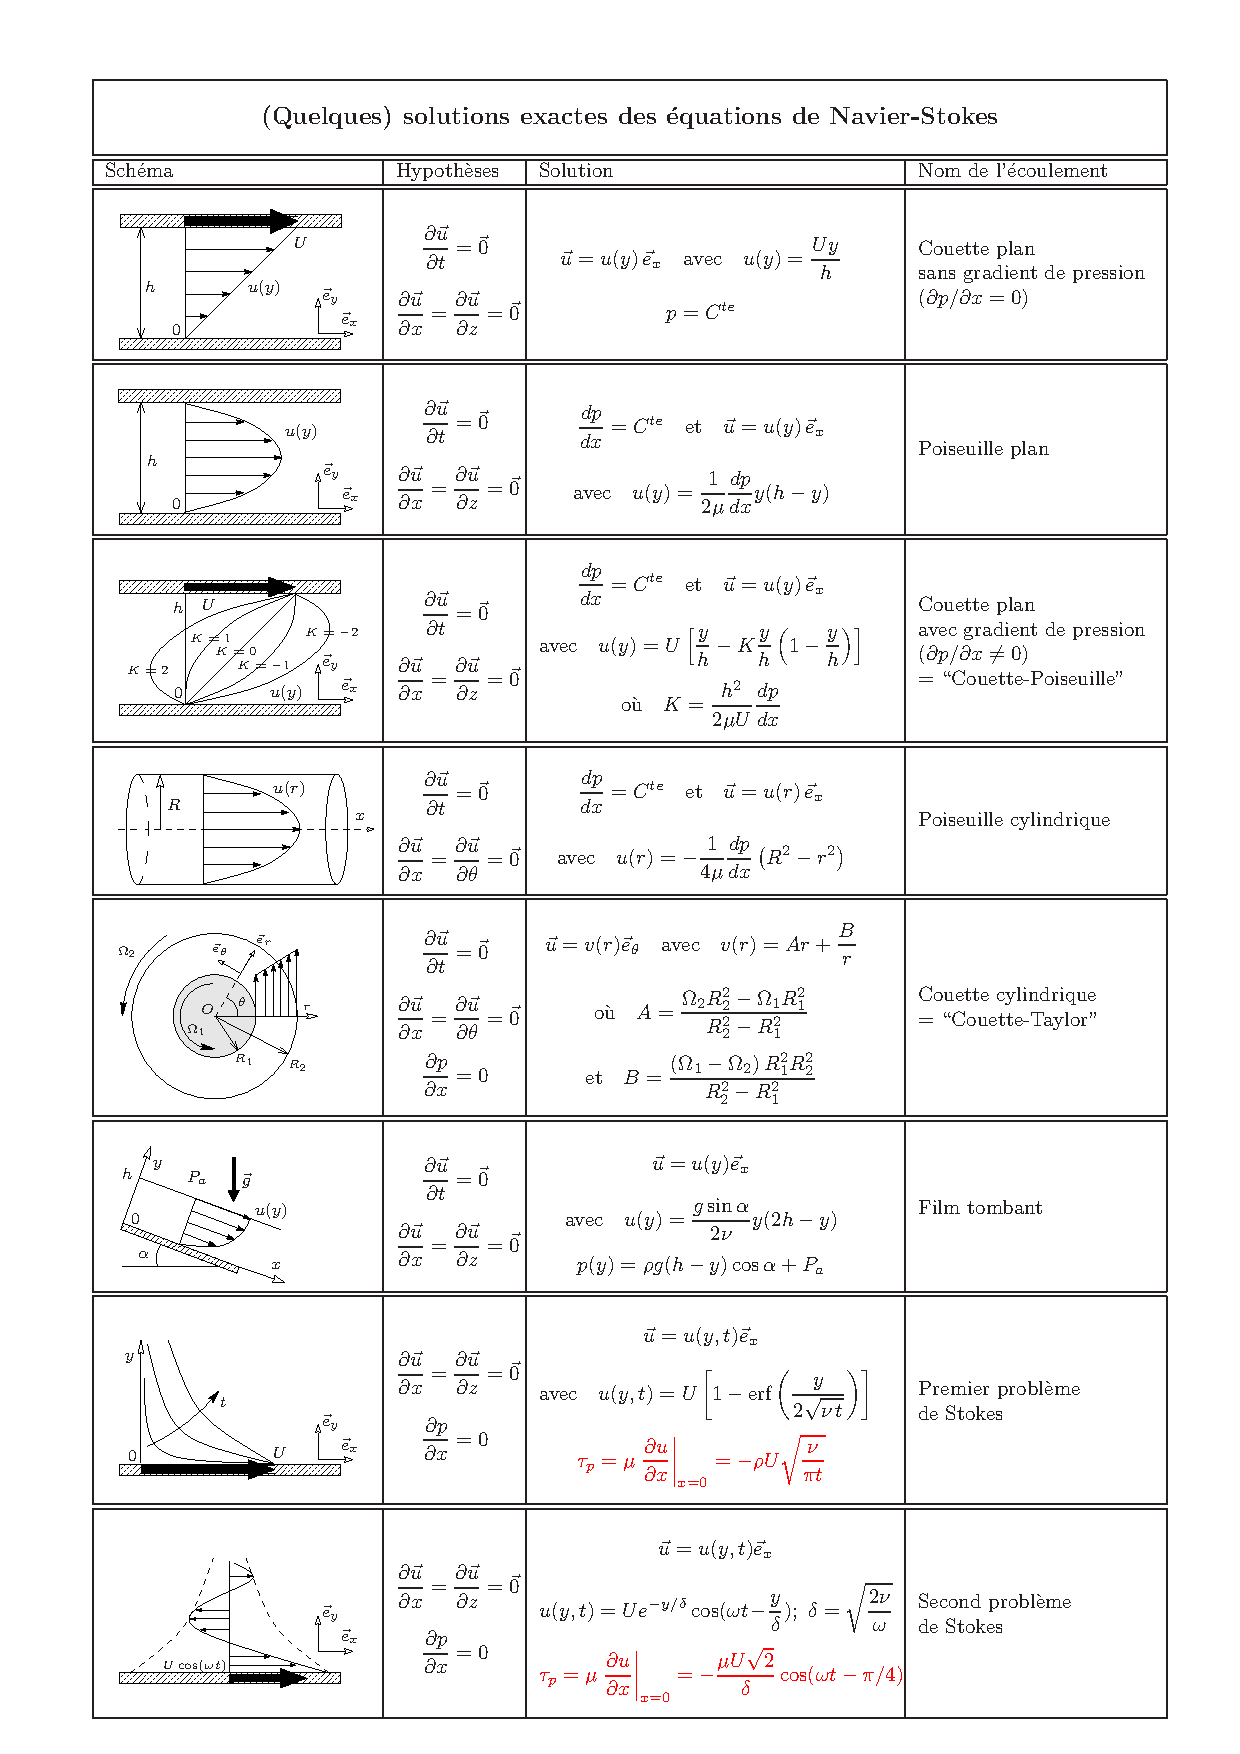
\includegraphics[height=27cm]{solutions_exactes_D}}
	\end{picture}
\end{center}


